% CHAPTER 9: Decoder during training
\chapter{Decoder Architecture during training}

Now that we have understood the different components used in the decoder, we will understand how they work together to make up the decoder of the transformer. As like in encoder, there is not one but 6 decoder blocks stacked up on top of each other. Each of the blocks has the same architecture but differ in their weights. A simplified representation of the decoder is provided below.
\begin{figure}[H]
    \centering
    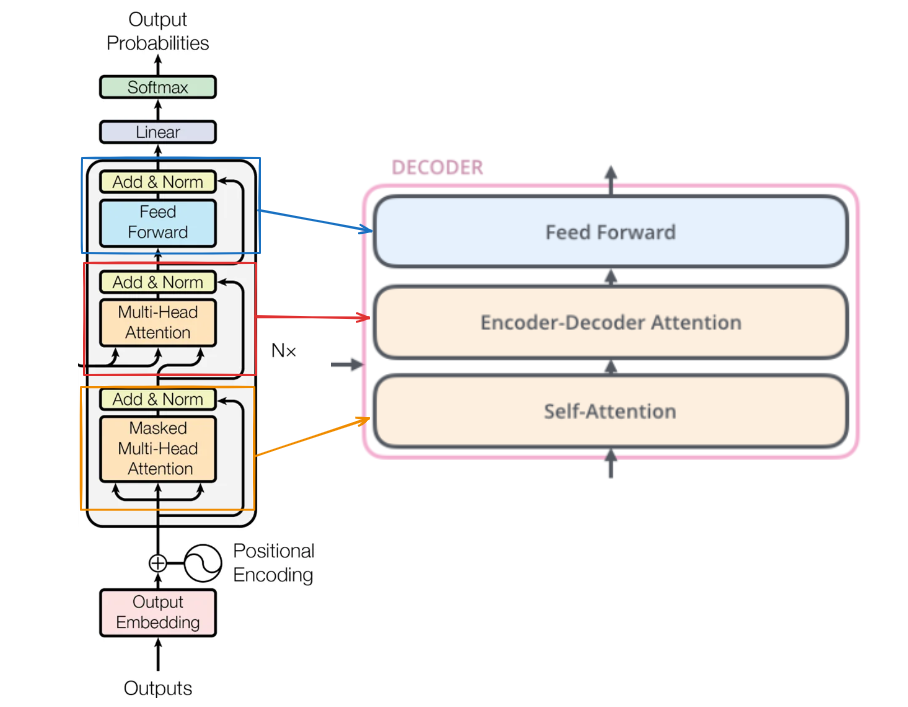
\includegraphics[width=0.6\linewidth]{Decoder-architecture-training/architecture-decoder.png}
    \caption{Decoder architecture in transformer}
\end{figure}

In the previous chapter on encoder, we generated the contextual embedding of the tokens (words) in the sentence \textbf{How are you?}. In Hindi, this translates to {\devanagarifont तुम कैसेहो?}. During the training period, this output is available to us and we feed this output as the input to the decoder. The subsequent sections will demonstrate how the input is processed in various parts of the decoder.

% Input of decoder
\section{The input}

The translated sentence from the output sequence (Hindi) is first right-shifted to add a token called \textbf{<start>}. This tells the decoder to start its task. Given below is a schematic diagram of how the input is processed before it enters the decoder block.
\begin{figure}[H]
    \centering
    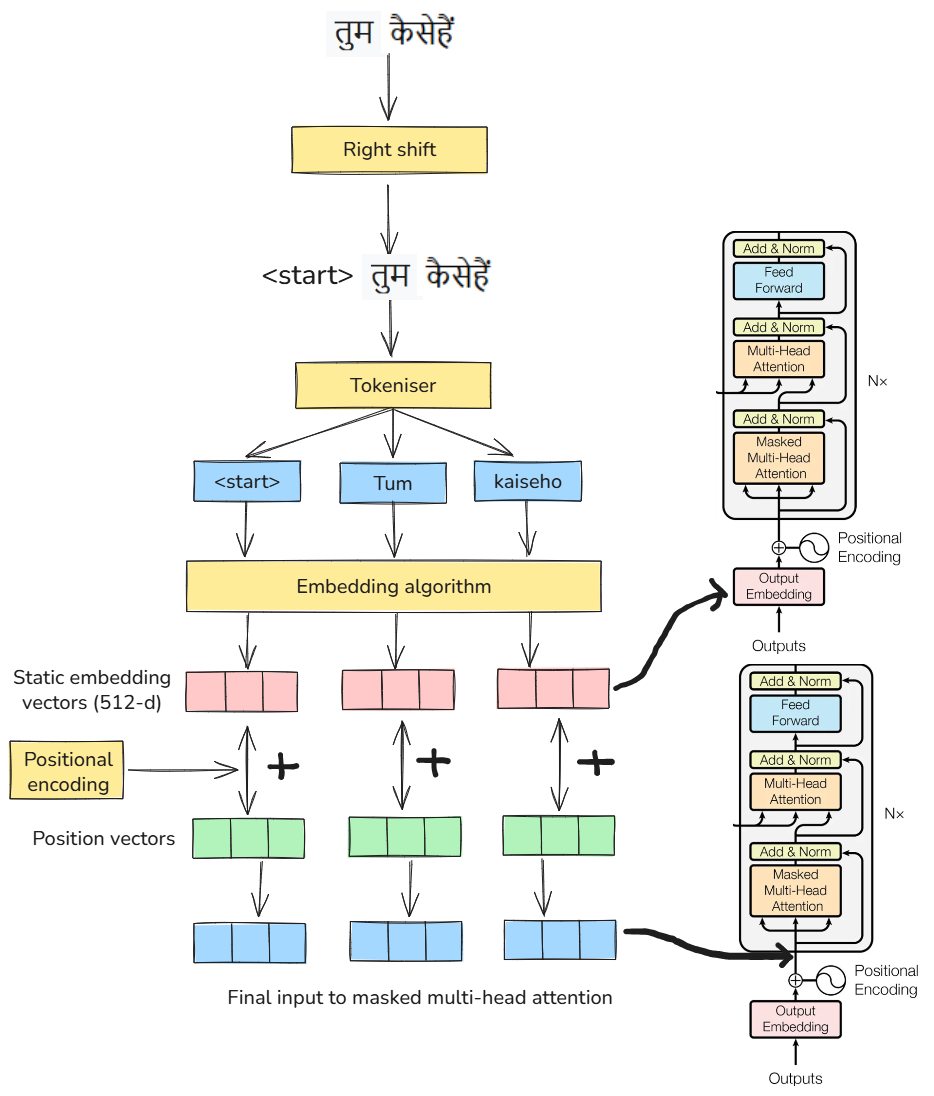
\includegraphics[width=0.75\linewidth]{Decoder-architecture-training/input-pe-decoder.png}
    \caption{Processing input before entering decoder}
\end{figure}

% Masked attention
\section{Masked multi-head attention and normalization}

The input obtained after positional encoding is passed on to the masked multi-head attention block. The output from that block and the input are added and normalized to give the output.
\begin{figure}[H]
    \centering
    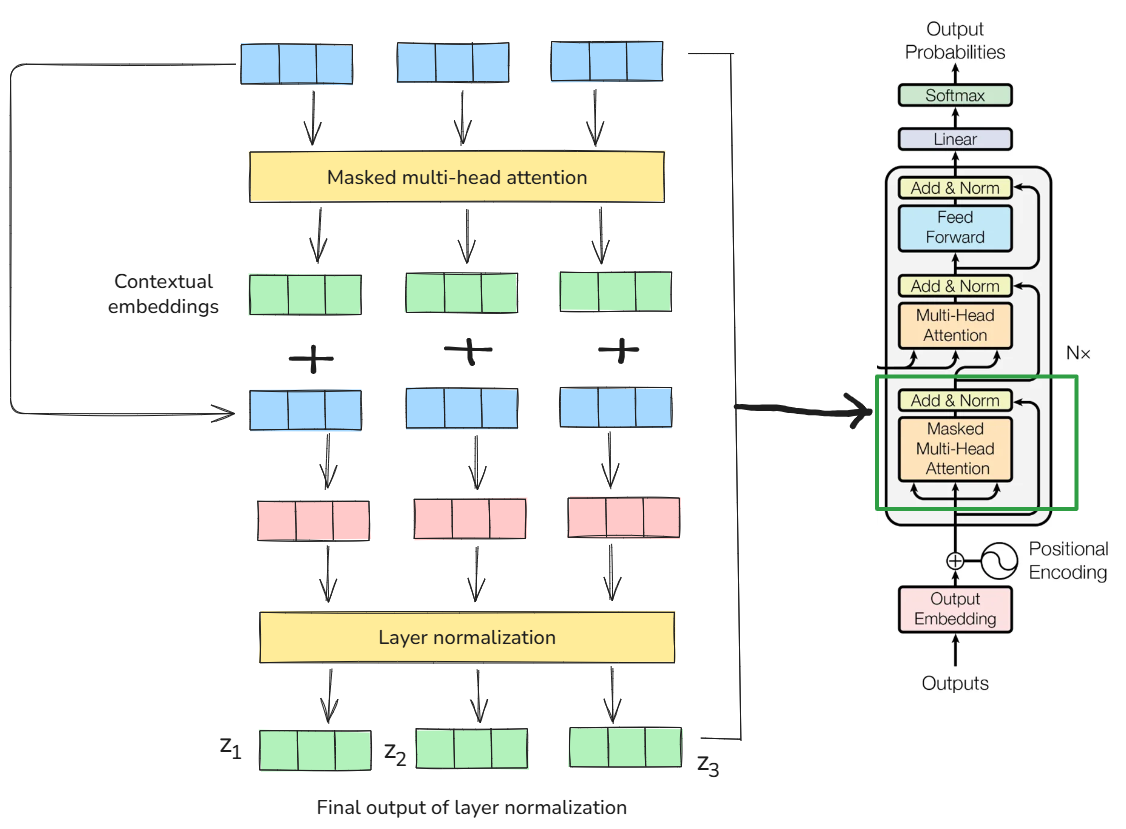
\includegraphics[width=0.75\linewidth]{Decoder-architecture-training/masked-multi-attention-decoder.png}
    \caption{Processing in the masked multi-attention block}
\end{figure}

% Cross attention
\section{Cross-attention and normalization}

The input obtained from layer normalization is sent into the cross-attention block. The vectors ($z_1$, $z_2$ and $z_3$) are multiplied by the query weight matrix ($W_q$) to generate the \textit{query} vectors. The \textit{key} and \textit{value} vectors are obtained from the encoder output by multiplying the encoder embeddings with the key weight matrix ($W_k$) and the value weight matrix ($W_v$), respectively. The output from this block and the input are added and normalized, to give the input for the FFNN.
\begin{figure}[H]
    \centering
    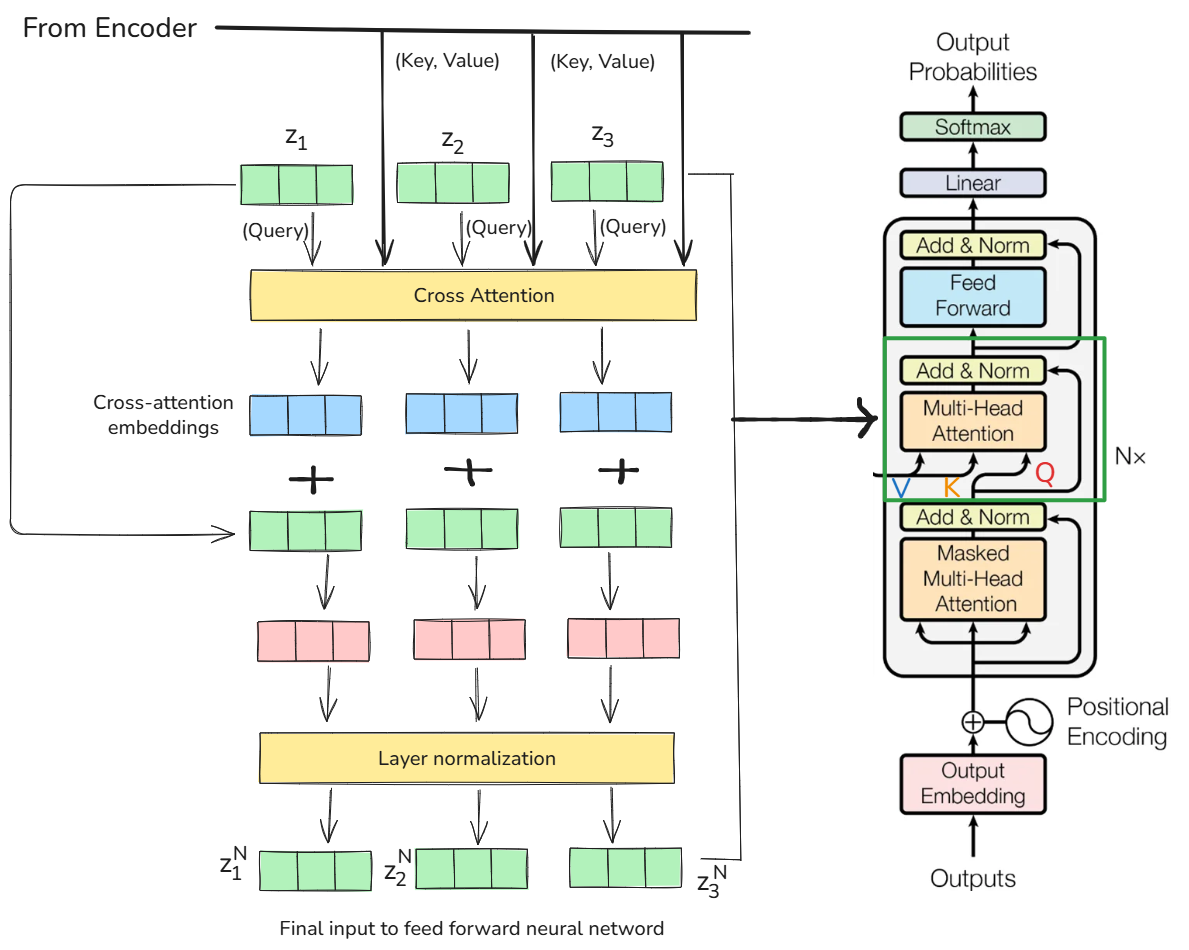
\includegraphics[width=0.75\linewidth]{Decoder-architecture-training/cross-attention-decoder.png}
    \caption{Processing in cross-attention block}
\end{figure}

% Feed forward NN
\section{Feed forward neural network}

The cross-attention block generates same number of vectors as input tokens. They are stacked up to create a matrix. Input into the FFNN goes in the form of "batches" of a fixed size. The FFNN has the same architecture as that of the encoder:
\begin{enumerate}
    \item \textbf{1 input layer} of 512 neurons.
    \item \textbf{1 hidden layer} of 2048 neurons (activation function - ReLU).
    \item \textbf{1 output layer} of 512 neurons (activation function - Linear).
\end{enumerate}

This was used in the original paper by the researchers. The architecture can be adjusted according to the specific use-case.
\begin{figure}[H]
    \centering
    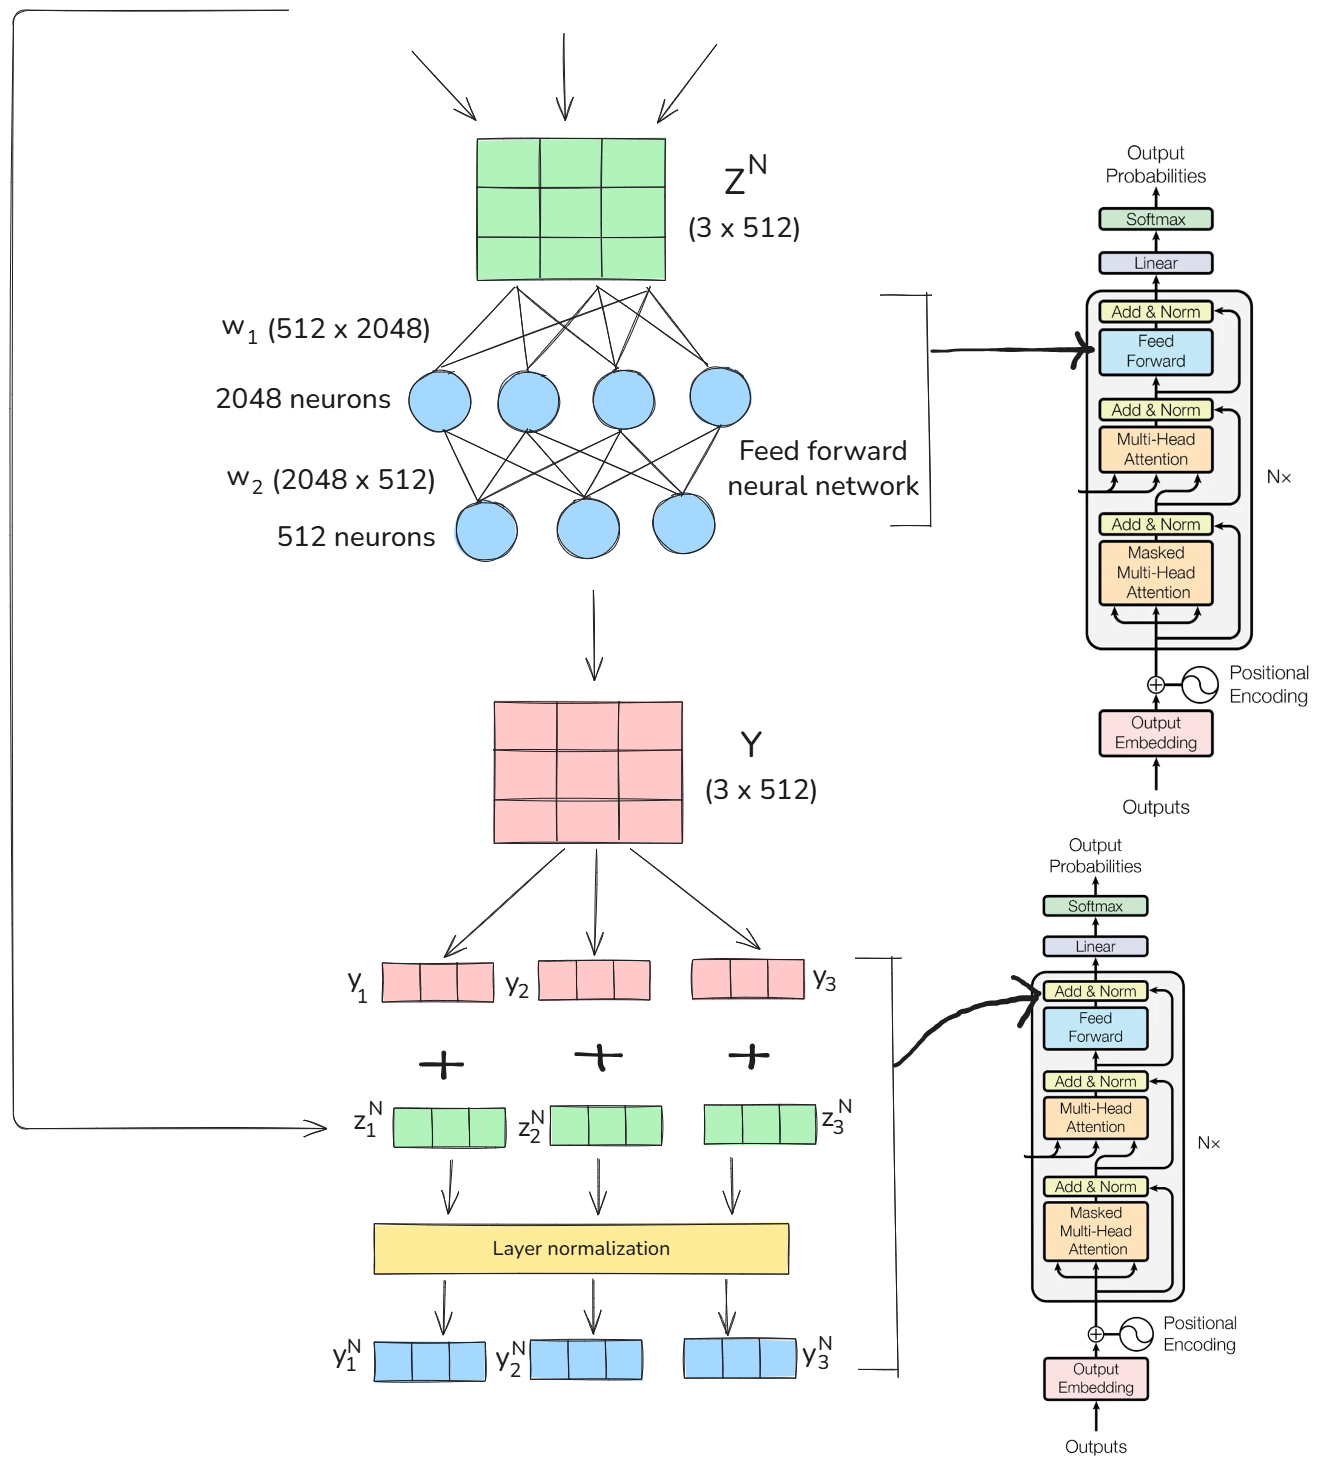
\includegraphics[width=0.75\linewidth]{Decoder-architecture-training/feed-forward-nn-decoder.png}
    \caption{Feed forward neural network}
    \label{fig:placeholder}
\end{figure}

% Output layer
\section{The output block}

The output from the FFNN and layer normalization layer goes through 5 other decoder blocks to produce the final output vectors - $y_1^f$, $y_2^f$ and $y_3^f$. They are again stacked up to form a matrix. These are then fed into another neural network in the form of "batches". The neural network has the following architecture:
\begin{enumerate}
    \item \textbf{1 input layer} of 512 neurons.
    \item \textbf{1 output layer} of $V$ neurons (activation function - softmax).
\end{enumerate}

$V$ is the number of unique words in the vocabulary of the output sequence (Hindi). For example, if the training dataset of the output sequence has the sentences ["We are friends", "How are you?"], then the unique words are ["We", "are", "friends", "How", "you"]. In that case, $V = 5$.

The softmax layer outputs a probability score for each of the words in the output sequence. The word having the maximum probability is selected as the output of the decoder.
\begin{figure}[H]
    \centering
    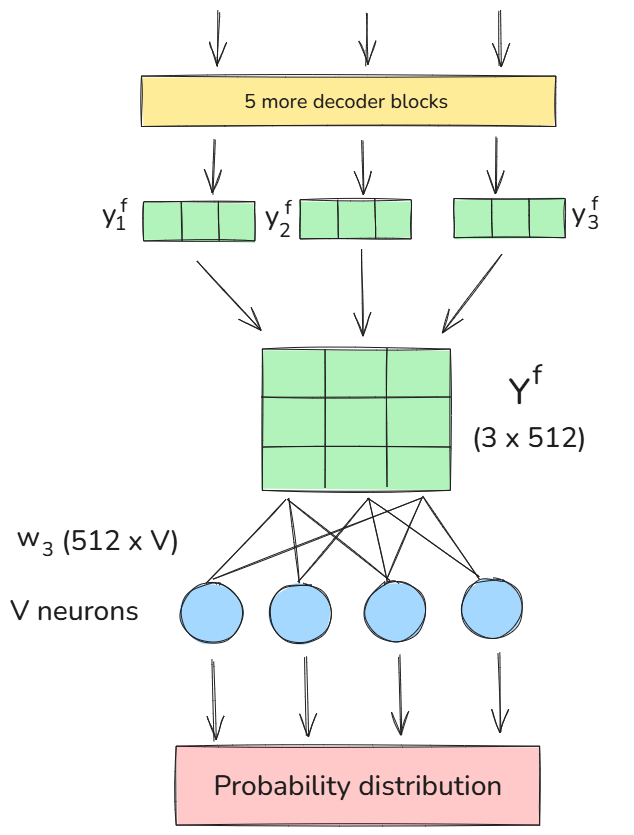
\includegraphics[width=0.5\linewidth]{Decoder-architecture-training/output-layer-decoder.png}
    \caption{Output layer in decoder}
\end{figure}

Let us say that for the vector representing the \textbf{<start>} token (1st vector in $Y_f$), the output from the network is {\devanagarifont तुम}. The next vector in $Y_f$ is for {\devanagarifont तुम}. For this input, let us say that the model predicts {\devanagarifont अच्छेहो} (which is wrong!). We do NOT pass this word as the next input to the network. Instead, we pass what was there in our original output sequence {\devanagarifont कैसेहो?} (which is the next vector in $Y_f$). This method is known as \textbf{teacher forcing}. During training, we use the tokens present in our output sequence, irrespective of whether the model predicts the correct output or not. This is the reason why the decoder behaves \textit{non-auto-regressively} during the training time, since it does not depend on the previous output for its next prediction.
\begin{figure}[H]
    \centering
    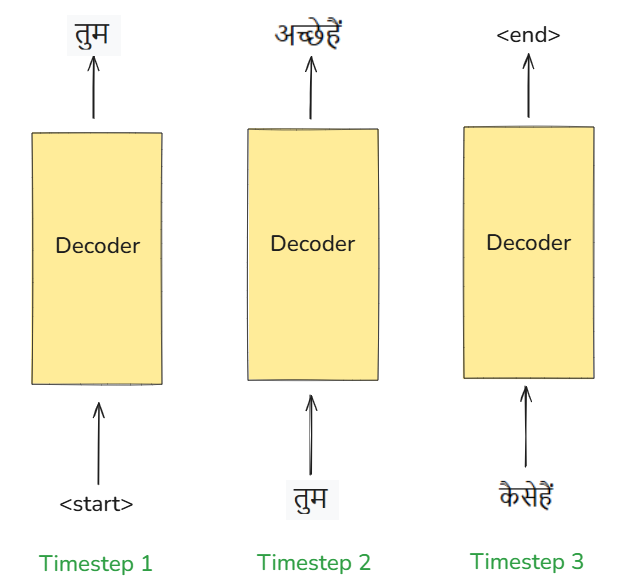
\includegraphics[width=0.5\linewidth]{Decoder-architecture-training/decoder-timestep.png}
    \caption{Teacher forcing in decoder during training}
\end{figure}

The decoder stops its task when it encounters a special \textbf{<end>} token. The entire decoder architecture can be viewed over \underline{\href{https://drive.google.com/file/d/1KNXPwZrg-DhPiqMJVMhhzh3kBte7yf4g/view?usp=drive_link}{here}}.

I hope this chapter was able to provide you with a good understanding of the working of the decoder during training. We are almost at the end of our journey of understanding the working of a transformer. In the next (and last!) chapter, we will discuss how the decoder works during inference.